\chapter{Prioritising Architectural Effort}
\label{chapter:prioritisation}

\section{Introduction}

In our practice in the field of software architecture, we have noticed and experienced how complex it is for software architects to prioritise their work.  The software architect's responsibilities are broad and, in principle, they can be involved in almost any technical aspect of a project from requirements to operational concerns.  In practice, this makes it difficult for an architecture practitioner to prioritise their effort to achieve quality properties like energy consumption, which acquiring stakeholders and end-users rarely prioritise explicitly due to their lack of immediate visibility.  Other important quality properties that suffer from similar prioritisation problems include security \cite{cisco2016-uksecprioritisation} and performance and availability \cite{ozkaya2008-qualityproperties}.

In the case of energy efficiency in particular, a previous survey of practitioners \cite{bashroush2016-datacentreenergy} revealed that the vast majority of them (83\%) admit that they do not prioritise energy efficiency as a key quality attribute of their systems but that a clear majority of them (67\%) thought that energy would be a key architectural concern in coming years.  There are likely to be a number of reasons for the current situation, including lack of stakeholder focus, the perception of limited tools and techniques for application energy usage, and the relative complexity of addressing application energy consumption, as it requires a multi-disciplinary approach to be effective.

However, our experience with other quality properties, particularly scalability and security, suggests that even when relevant tools exist and there is general acceptance that the qualities are important, architects (and development teams more generally) often find it difficult to prioritise these concerns against short term priorities such as feature completion, fixing defects and performance fixes that address usability concerns.  While it is important to address these immediate concerns, they are short-term solutions, which do not improve the fundamental quality of the system that determines its long term viability. 

While addressing fundamental, rather than short-term, concerns is challenging, we observe that successful experienced software architects appear to be able to do this.  These experienced architects are good at focusing their effort for maximum long-term effect, and manage to create performant, secure, highly available systems, and we hope in the future, energy efficient systems too. However not all architects have this skill and anecdotally we observe that inexperienced architects often find prioritising effort very difficult.  This situation led us to wonder how the experienced architects achieve their balance between immediate and long-term concerns.  As discussed in \sref{section:litreview-prioritisation}, there is little to guide them in the existing research literature, although they may use simple techniques like ad-hoc prioritisation or numeric grouping.  They may also use generic time management techniques (like \cite{allen2015-gettingthingsdone}) but we were interested in whether there are common role-specific heuristics which could be taught to new architects.

We decided to investigate this via a questionnaire-based study of a group of experienced architects.  We discovered that there are common heuristics which experienced architects use to prioritise their work and we created a model to capture them.  We then validated the model via an online questionnaire with a much wider group of practitioners and refined the model based on their input.

In this chapter, we explain the approach we took and present both the initial model that we created from the results of the interview process and the final, refined, model that we created after the validation process.  The contribution of the work is not specifically the heuristics in the model, indeed most of them are quite familiar to experienced practitioners, but rather the organisation of the heuristics and the validation that they are used by experienced practitioners to guide their work.  We believe that this makes the model a useful reminder for experienced practitioners and an effective teaching aid for new architects who are learning how to perform the role.

\section{Research Method}

When planning this research, we selected a qualitative research approach because we needed to explore the "lived-experiences" of expert practitioners by asking them questions to encourage reflection and insight \cite{lapan2012-qualitativeresearch} rather than assessing performance or alignment with specific practices via quantitative means.

The process was organised into four distinct stages.

\begin{description}
	\item [Stage 1] gathering primary data using semi-structured interviews with practitioners.
	\item [Stage 2] analysis of the primary data and creation of a preliminary model.
	\item [Stage 3] validation of the preliminary model via a structured online questionnaire, completed by practitioners in relevant architecture roles (primarily software, solution and enterprise architects).
	\item [Stage 4] analysis of the validation data and refinement of the preliminary model into a final, validated model.
\end{description}

We chose to gather our primary data using semi-structured interviews, where we provided the interviewees with a written introduction to the question we wanted to answer and then some specific questions to start their thought processes. 

The analysis of the primary data was performed using a simple application of Grounded Theory as it is a suitable method for theory building, to understand the relationships between abstract concepts \cite{charmaz2006-groundedtheory}, which described our situation and needs very closely.  We performed initial coding on the primary data and then refined this with a more focused coding exercise.  As suggested in \cite{lapan2012-qualitativeresearch}, the process of collection and analysis was a parallel, iterative process, rather than a linear one with fixed phases.  

This exercise produced a set of themes that classify the heuristics that the architects use, as well as the heuristics themselves.  A heuristic had to be mentioned by at least three of the participants (which represented a third of them) for us to consider it significant enough to be included in the model.  We combined the themes and heuristics to form a simple model (the "preliminary model") of how experienced architects go about prioritising their effort. 

Once we had the preliminary model available, we published it at a research conference \cite{woods2017-archpriorisation} and via a LinkedIn post (https://www.linkedin.com/pulse/focusing-software-architects-attention-eoin-woods) and created an online questionnaire \cite{gillham2000-questionnaire} aimed at architecture practitioners to allow them to evaluate and comment on the usefulness of the model.  We publicised the survey via LinkedIn, Twitter and via direct email to our network of architecture practitioners.

We received 84 responses to the survey, containing answers to our closed-ended questions to evaluate the usefulness of the model and also received answers to open-ended questions in 50 of the responses.  We used the closed-ended questions to evaluate the usefulness of the model and analysed the open-ended responses to identify themes which needed to be addressed by the model.

The model was validated strongly across respondents from different locations, with different amounts of experience and from different architectural specialisations. Additionally, a small number of themes emerged from the answers to the open-ended questions.  These themes for improving the model were used to revise and extend it slightly, creating an improved final version that reflected the input from the respondents.

A description of the four stages of the research method is presented below, along with the final version of the architectural effort prioritisation model.

\section{Stage 1 - The Initial Study}
\label{section:initialstudy}

Our primary data gathering was performed using a semi-structured, face-to-face survey of 8 experienced software architecture practitioners working across 4 countries.

We found the participants by approaching suitable individuals from our professional networks.  We were looking for practitioners who had a minimum of 10 years' professional experience and who worked as architects in the information systems domain (rather than architects from \textendash for example \textendash embedded systems).  

We focused on the information systems domain because we know from experience that working practices differ between professional domains like information systems and embedded systems.  Hence, we thought it was more likely that we could create a useful model if we limited ourselves to one broad domain, at least initially. 

We deliberately selected candidates that we knew differed from each other in organisation, specialisation and geography to get a reasonably diverse population and avoid obvious sample bias (we discuss the threat of sample bias further in Section \ref{sec:threats}).

Some characteristics of the participants in the study are summarised in the graphs in Figure \ref{figure:participants}.  As can be seen, they represent a range of experience, role type and country.

%%
%% See this page for the magic:
%% https://tex.stackexchange.com/questions/64858/how-to-create-subfloat-figures-two-in-first-row-and-one-below
%%
%%       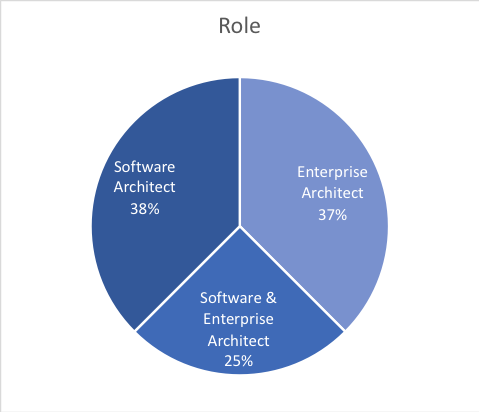
\includegraphics[scale=0.9, trim=5 5 5 5,clip]{Figures/prioritisation-roles}

\begin{figure}
   \begin{subfigure}{.5\linewidth}
      \centering
      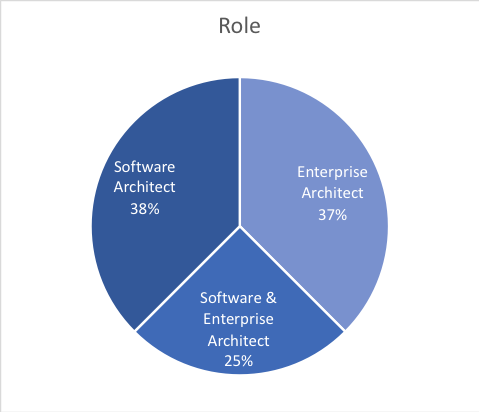
\includegraphics[scale=1.0]{Figures/prioritisation-roles}
   \end{subfigure}
   \begin{subfigure}{.5\linewidth}
      \centering
      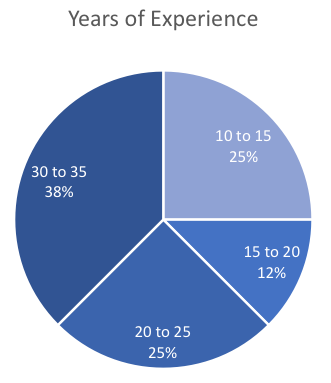
\includegraphics[scale=1.0]{Figures/prioritisation-yearsexp}
   \end{subfigure}
   \begin{subfigure}{\linewidth}
      \centering
      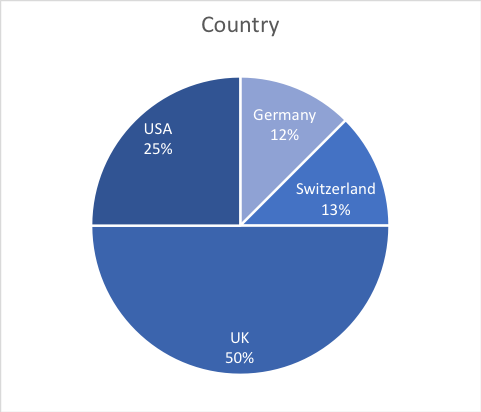
\includegraphics[scale=1.0]{Figures/prioritisation-countries}
   \end{subfigure}

   \caption{Study Participants (8 in total)}
   \label{figure:participants}
\end{figure}  

All of the members of our initial practitioner set had over 10 years of post-graduate experience and some had over 30 years of experience, so ensuring that they all had a significant amount of professional practice upon which to base their answers.

We deliberately selected software and enterprise architects because this is whom the model was primarily aimed at serving.

We approached individuals in a number of countries to try to minimise the risk that we would reflect practice only in one country, although we did not manage to gain representation from beyond North America and Europe.

We used a semi-structured interview format with a written introduction to the question which each interviewee read before being asked a standard set of open-ended questions which explored how they went about prioritisation of architecture work and any specific factors that they used to guide them.  

The question we asked was "how can the architect concentrate their attention so that they are most effective?" The more specific questions used to stimulate the thought process were: 

\begin{itemize}
	\item How do you go about this in your work? 
	\item What factors do you consider when prioritising your attention? 
	\item Do you consider what to focus on?   Or what not to focus on? 
	\item For example, how do you prioritise architectural governance compared to other aspects of the project?
\end{itemize}

The interviewer asked additional questions to understand the answers fully or to encourage the interviewee to add more detail or fill in ambiguous aspects of the answer.

The process of initial coding of the primary data resulted in 25 items, which could be associated with at least one of the interviews.  A further focused coding process revealed that there were 9 underlying heuristics which appeared to be significant to the participants in the study. Then, a further analysis iteration lead to the identification of three categories of prioritisation heuristic which we use to structure our model.

\section{Stage 2 - Preliminary Model for Prioritising Architectural Effort}
\label{section:prelim-model}

\subsection{The Preliminary Model}

Our preliminary heuristic model for focusing architectural effort is shown in Figure \ref{figure:prelmodel}.
 
The three categories of heuristic that the study revealed were: first, the need to focus on stakeholder needs; second, the importance of considering risks when deciding on where to focus effort; and finally the importance of spending time to achieve effective delegation of responsibilities.  These categories form the structure of our model and remind the architect of the general ways in which they should prioritise their efforts. The categories and heuristics are explained in more detail in section \ref{sec:prelim-model-content}.

\begin{figure}
\centering

\includegraphics[width=\textwidth]{Figures/prioritisation-prelim-model}
\caption{Preliminary Model for Focusing Architectural Attention}
\label{figure:prelmodel}
\end{figure}  

It is important to understand the nature of this model and how it should be used.  It is not a prescriptive process for architects to follow or a process for developing an architecture.  This model is an aide memoir to organise and present a set of heuristics that experienced architecture practitioners appear to find useful when prioritising their work.  While we believe this to be a useful model to teach trainee architects and a useful reminder for experienced architects, it is necessary to apply the model in a context-sensitive manner, within whatever method that the architect is using to develop software architectures.

\subsection{Content of the Preliminary Model}
\label{sec:prelim-model-content}

\subsubsection{Understand the Stakeholder Needs and Priorities}

The first theme which emerged strongly in our study was focusing on the needs and priorities of the stakeholders involved in the situation.  The principle that architecture work involves working closely with stakeholders is widely agreed upon \cite{rozanski2011-ssa2e, bass2012-sainp} and this theme reinforces that. Architects need to focus significant effort to make sure that stakeholder needs and priorities are understood to maximise focus on the critical success factors for a project and maximise the chances of its timely completion.  Based on the study, three specific heuristics to achieve this were identified:

\begin{itemize}
	\item \emph{Consider the whole stakeholder community}. Spend time understanding the different groups in the stakeholder community and avoid the mistake of just considering obvious stakeholder groups like end-users, acquirers and the development team.  As the architecture methods referenced above note, ignoring important stakeholders (like operational staff or auditors) can prevent the project from meeting its goals and cause significant problems on the path to production operation.
	\item \emph{Ensure that the needs of the delivery team are understood and met}.  Spend sufficient time to ensure that the delivery team can be effective.  What is the team good at?  What does it know?  What does it not know?  What skill and knowledge gaps does it have?  These areas need attention early in the project so that architecture work avoids risks caused by the capabilities of the team and that time is taken to support and develop the team to address significant weaknesses.
	\item \emph{Understand the perspective and perceptions of the acquirers of the system}.  Acquirers are a key stakeholder group who judge its success and usually have strategic and budgetary control, so can halt the project before delivery if they are unhappy.  Specifically addressing this group's needs, perceptions and concerns emerged as an important factor for some of the experienced architects in our study.  Acquirers are often distant from the day-to-day reality of a project and need clear communication to understand their concerns and ensure that they have a realistic view of the project.
\end{itemize}

\subsubsection{Prioritise Effort According to Risks}

During a project, an effective approach to prioritising architectural attention is to use a risk-driven approach to identify the most important tasks.  If the significant risks are understood and mitigated, then enough architecture work has probably been completed.  If significant risks are open, then more architecture work is needed. The specific heuristics to consider for risk assessment are:

\begin{itemize}
	\item \emph{Consider external dependencies}.  Understand your external dependencies because you have little control over them and they need architectural attention early in the project and whenever things change.
	\item \emph{Look for novel aspects of domain, problem and solution}.  Another useful heuristic, from the experience of our study participants, is to focus on novelty in your project.  What is unfamiliar?  What problems have you not solved before?  Which technology is unproven?  The answers to these questions highlight risks and the participants in our study used them to direct their effort to the most important risks to address.
	\item \emph{Identify the high impact decisions}.  Prioritise architecture work that will help to mitigate risks where many people would be affected by a problem (e.g. problems with the development environment or problems that will prevent effective operation) or where the risk could endanger the programme (e.g. missing regulatory constraints).
	\item \emph{Analyse your local situation for risks}.  Consider the local factors unique to your situation, which you will be aware of due to the knowledge you have of the domain, problem and solution.  It is impossible to give more specific guidance on this heuristic as every situation is different, but the participants in our study noted the importance of "situational awareness" \cite{wikipedia-sitawareness} that allows the architect to find and address the risks specific to the local environment (perhaps due to organisational factors, specific technical challenges, domain complexities or business constraints).
\end{itemize}

\subsubsection{Delegate as Much as Possible}

Delegation was an unexpected theme that emerged from our study. The architects who mentioned this theme viewed themselves as a potential bottleneck in a project and delegation and empowerment of others was a way to minimise this.  Delegation was also seen as a way of freeing the architect to focus on the aspects of the project that they had to focus on rather than all the other aspects that they could possibly get involved in.

The general message of this theme is to delegate as much architecture work as possible to the person or group best suited to perform it, to prevent individuals becoming project bottlenecks, allow architects to spend more time on risk identification and mitigation, and to spread architectural knowledge through the organisation.  The heuristics that were identified to help achieve this are:

\begin{itemize}
	\item \emph{Empower the development teams}. To allow delegation and work sharing, architects need to empower (and trust) the teams they work with.  This allows governance to become a shared responsibility and architecture to be viewed as an activity rather than something that is only performed by one person or a small group.  This causes architectural knowledge, effort and accountability to be spread across the organisation, creates shared ownership, reduces the load on any one individual and prevents reliance on a single individual from delaying progress.
	\item \emph{Create groups to take architectural responsibilities}.  A related heuristic is to formalise delegation somewhat and create groups of people to be accountable for specific aspects of architectural work.  For example, in a large development programme, an architecture review board can be created to review and approve significant architectural decisions.  Such a group can involve a wide range of expertise from across the programme and beyond, so freeing a lead architect from much of the effort involved in gathering and understanding the details of key decisions, while maintaining effective oversight to allow risks to be controlled and technical coherence maintained.  Similarly, a specific group of individuals could be responsible for resilience and disaster recovery for a large programme, allowing them to specialise and focus on this complex area, and allowing a lead architect to confidently delegate to them, knowing that they will have the focus and expertise to address this aspect of the architecture.
\end{itemize}

\section{Stage 3 - Validating the Preliminary Model}
\label{sec:validating-prelim-model}
\subsection{The Questionnaire}

Once we had a preliminary model, we wanted to validate its usefulness with a much larger group of experienced practitioners.  This was conducted using a structured online questionnaire.  The questionnaire asked the respondents to read the model and then comment on its credibility and usefulness.  We asked both closed questions, that asked respondents to rate the model on 5 point scales, and open-ended questions that allowed the respondents to consider whether there were aspects of focusing attention that we had missed and also to collect general comments on the model.  Finally, we asked some closed classification questions to allow us to understand who had completed the survey while preserving their anonymity if desired.

We asked three closed-ended questions to find out whether the respondent thought that the model was credible and useful.  These questions and the possible responses were:

\begin{description}
	\item [Q1] "Is this model similar to how you focus architectural attention in your work already?" (Not at all similar / Not Very Similar / Somewhat Similar / Quite Similar / Very Similar)
	\item [Q2] "Would you find this model helpful in guiding architectural attention for maximum benefit?" (Definitely Not / Probably Not / Possibly / Probably Yes / Definitely Yes)
	\item [Q3] "Are the areas of risk mentioned in the "Prioritise time according to risks" activity valuable?" (Definitely Not / Probably Not / Somewhat / Probably Yes / Definitely Yes)
\end{description}

The open-ended questions that we asked were:

\begin{description}
	\item [Q4] "Are there other general areas of risk that should be added to 'Prioritise time according to risks' that would be applicable to most (information) systems and environments? If so please list and briefly explain them."
	\item [Q5] "Are there any significant factors missing from the model which you use to focus your architectural work?"
	\item [Q6] "Do you have any other comments on the  model or the survey"
\end{description}

The closed-ended questions we asked to allow us to classify the respondents and their possible answers were:
\begin{description}
   \item [Q7] "What environment do you work in?"
	\begin{itemize}
		\item Industry (developing systems, consultancy and related work)
		\item Industrial Research (working in a research environment for an industrial employer) 
		\item Academic (teaching or researching in university or similar environments)
		\item Other (please specify)
	\end{itemize}
	\item [Q8] How many years of post-graduation experience do you have?   
   \begin{itemize}
		\item 1-5 years
		\item 5-10 years
		\item 10-15 years
		\item 15-20 years
		\item More than 20 years
    \end{itemize}
   \item [Q9] What is your main job role? \nolinebreak
	\begin{itemize}
		\item Software Architect
		\item Enterprise Architect
		\item Software Designer
		\item Researcher
		\item Other (please specify)
    \end{itemize}
	\item [Q10] Where in the world are you based?
	\begin{itemize}
		\item North America
		\item South America 
		\item Europe (including the UK) 
		\item Middle-East and Africa 
		\item Asia-Pacific
		\item Other (please specify)
	\end{itemize}
\end{description}

We also invited them to leave an email address if they wanted to be informed of the outcome of the study and provided a free text box for any final comments or questions.  We did not view the email address and the final text box as survey data for the purposes of analysis.

Having trialled the questionnaire ourselves and with two other individuals, we expected most respondents to take 10 - 15 minutes to complete it.

\subsection{The Respondents}

To use the questionnaire to validate the model, we needed to find a suitable set of architects who could read it and complete the survey for us.  We found our respondents via two main activities.  
Firstly, we created a LinkedIn post \footnote{https://www.linkedin.com/pulse/focusing-software-architects-attention-eoin-woods} which provided an outline of the model, explained that we wanted to validate it and whom we wanted to participate, and provided a link to the survey.  This was posted from my account and so tended to appear in the LinkedIn news feed of practitioners, as my LinkedIn network contains many more practitioners than researchers.  The post was further publicised via Twitter and Facebook to reach a larger audience.  This step was moderately successful, with the post being viewed about 700 times and about 25 people completing the survey successfully.

To gain more responses to the survey, the second activity was a targeted email sent to individuals that we knew personally and whom we knew were practising software related architects (including software, solution and enterprise architects).  This second activity resulted in about 60 more responses to the survey.

In total, we received 84 completed surveys.

The job roles of the respondents are summarized in Figure \ref{figure:resproles}.  About a third of the respondents identified themselves as software architects, about a quarter as enterprise architects, about 12\% as software designers, 10\% as solution architects, and 5\% as technical architects.  Four respondents did not complete this answer and four had other job titles (a risk assessor, a technical manager and systems engineer, a project manager and a strategy consultant).

\begin{figure}
\centering
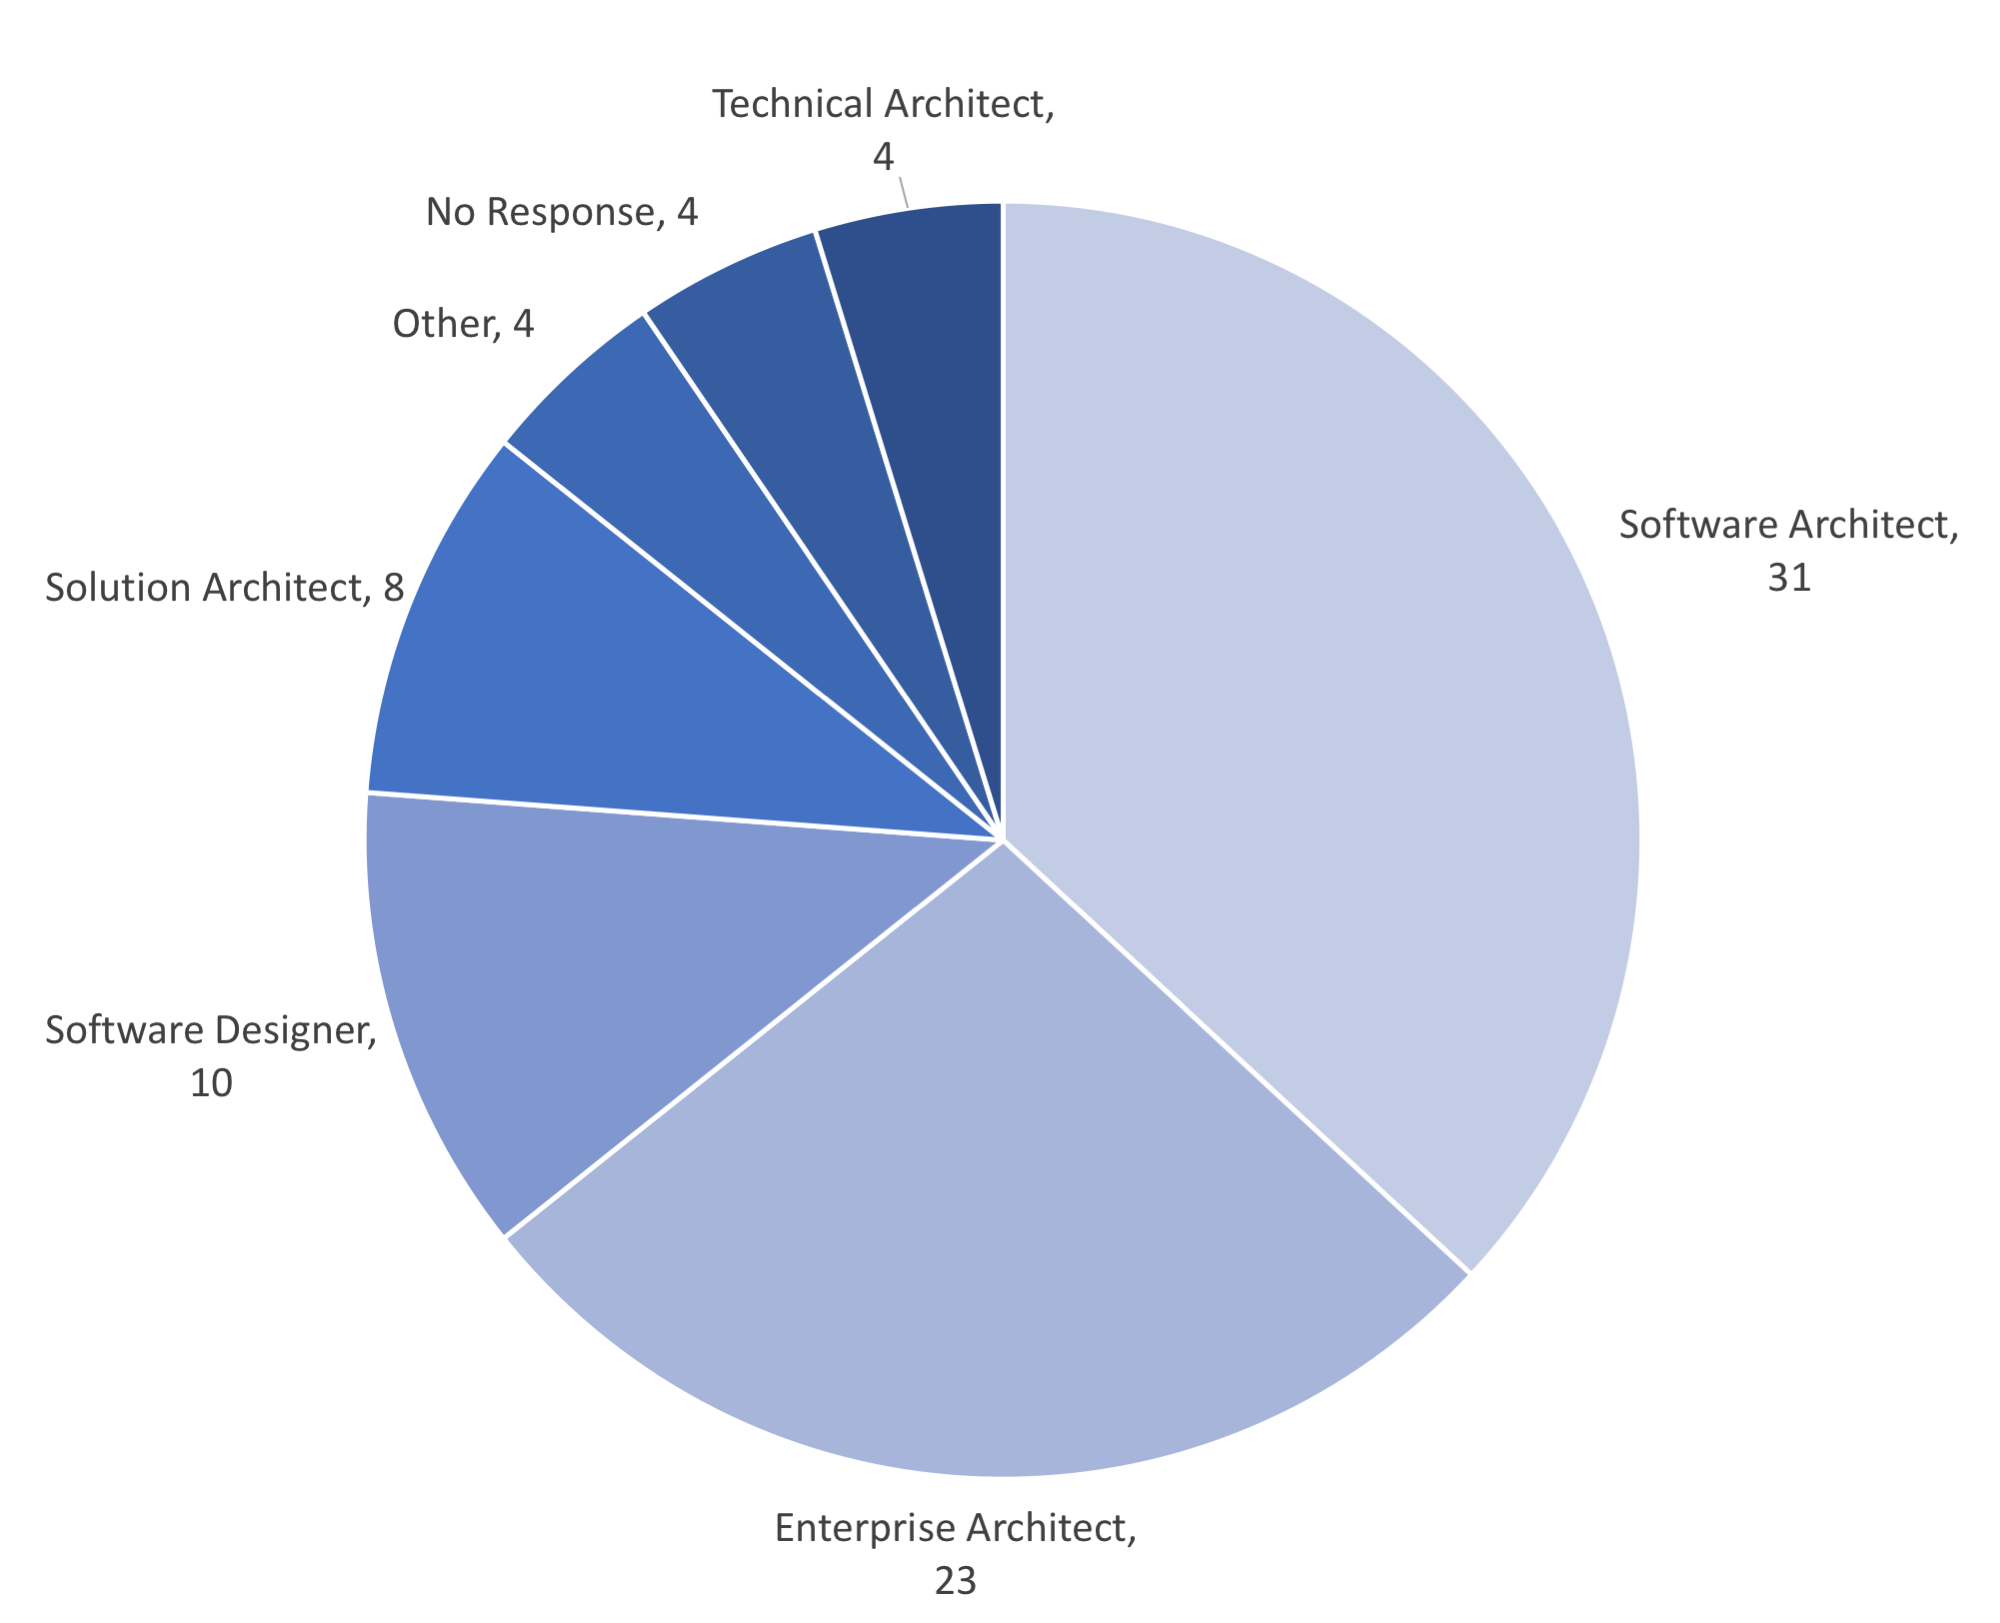
\includegraphics[width=8cm,trim={2 2 2 2},clip]{Figures/prioritisation-detailed-roles}
\caption{Respondent Roles}
\label{figure:resproles}
\end{figure}


The work environments of the respondents were overwhelmingly industrial (we viewed those building systems in the public sector as part of "industry"), with only one respondent having a purely academic work environment.  Five respondents did not provide an answer to this question.  Of these five, two were from German IP addresses, one Swiss and two UK addresses.  Four were from private ISP connections and one was from a UK public sector body, which, with another respondent who identified themselves as working in the public sector, suggested there were at least two public sector respondents.
 
\begin{figure}
\centering
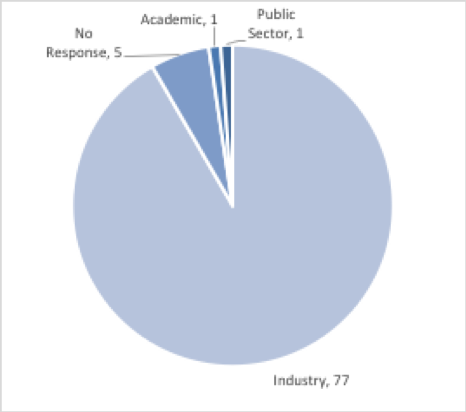
\includegraphics[width=6cm,trim={2 2 2 2},clip]{Figures/prioritisation-workenv}
\caption{Respondent Work Environments}
\label{figure:workenvs}
\end{figure}

We had some geographical distribution of respondents, as shown in Figure \ref{figure:geographies}, although there is a clear bias towards Europe, almost certainly caused by our professional networks being centred in Europe.  55\% of respondents identified themselves as coming from Europe, 30\% from the Americas and only 7\% from Asia-Pacific and a single correspondent from the Middle-East and Africa.

\begin{figure}
\centering
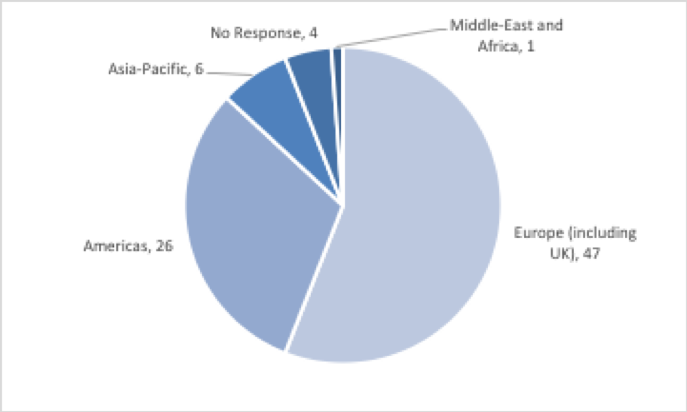
\includegraphics[width=8cm,trim={2 2 2 2},clip]{Figures/prioritisation-regions}
\caption{Respondent Geographies}
\label{figure:geographies}
\end{figure}

To delve a little deeper, we checked the geographical location of the respondents' IP addresses using the well-known "geoiplookup" command line tool \footnote{http://geoiplookup.net}.  Of the four respondents who did not answer the question, the IP addresses they were using were in the UK (two), Germany (one) and Switzerland (one).  While this does not prove that the respondents work in those countries (they could have been travelling away from home) it does make it likely that they are from Europe, taking the European percentage to about 60\%.
 
\begin{figure}
\centering
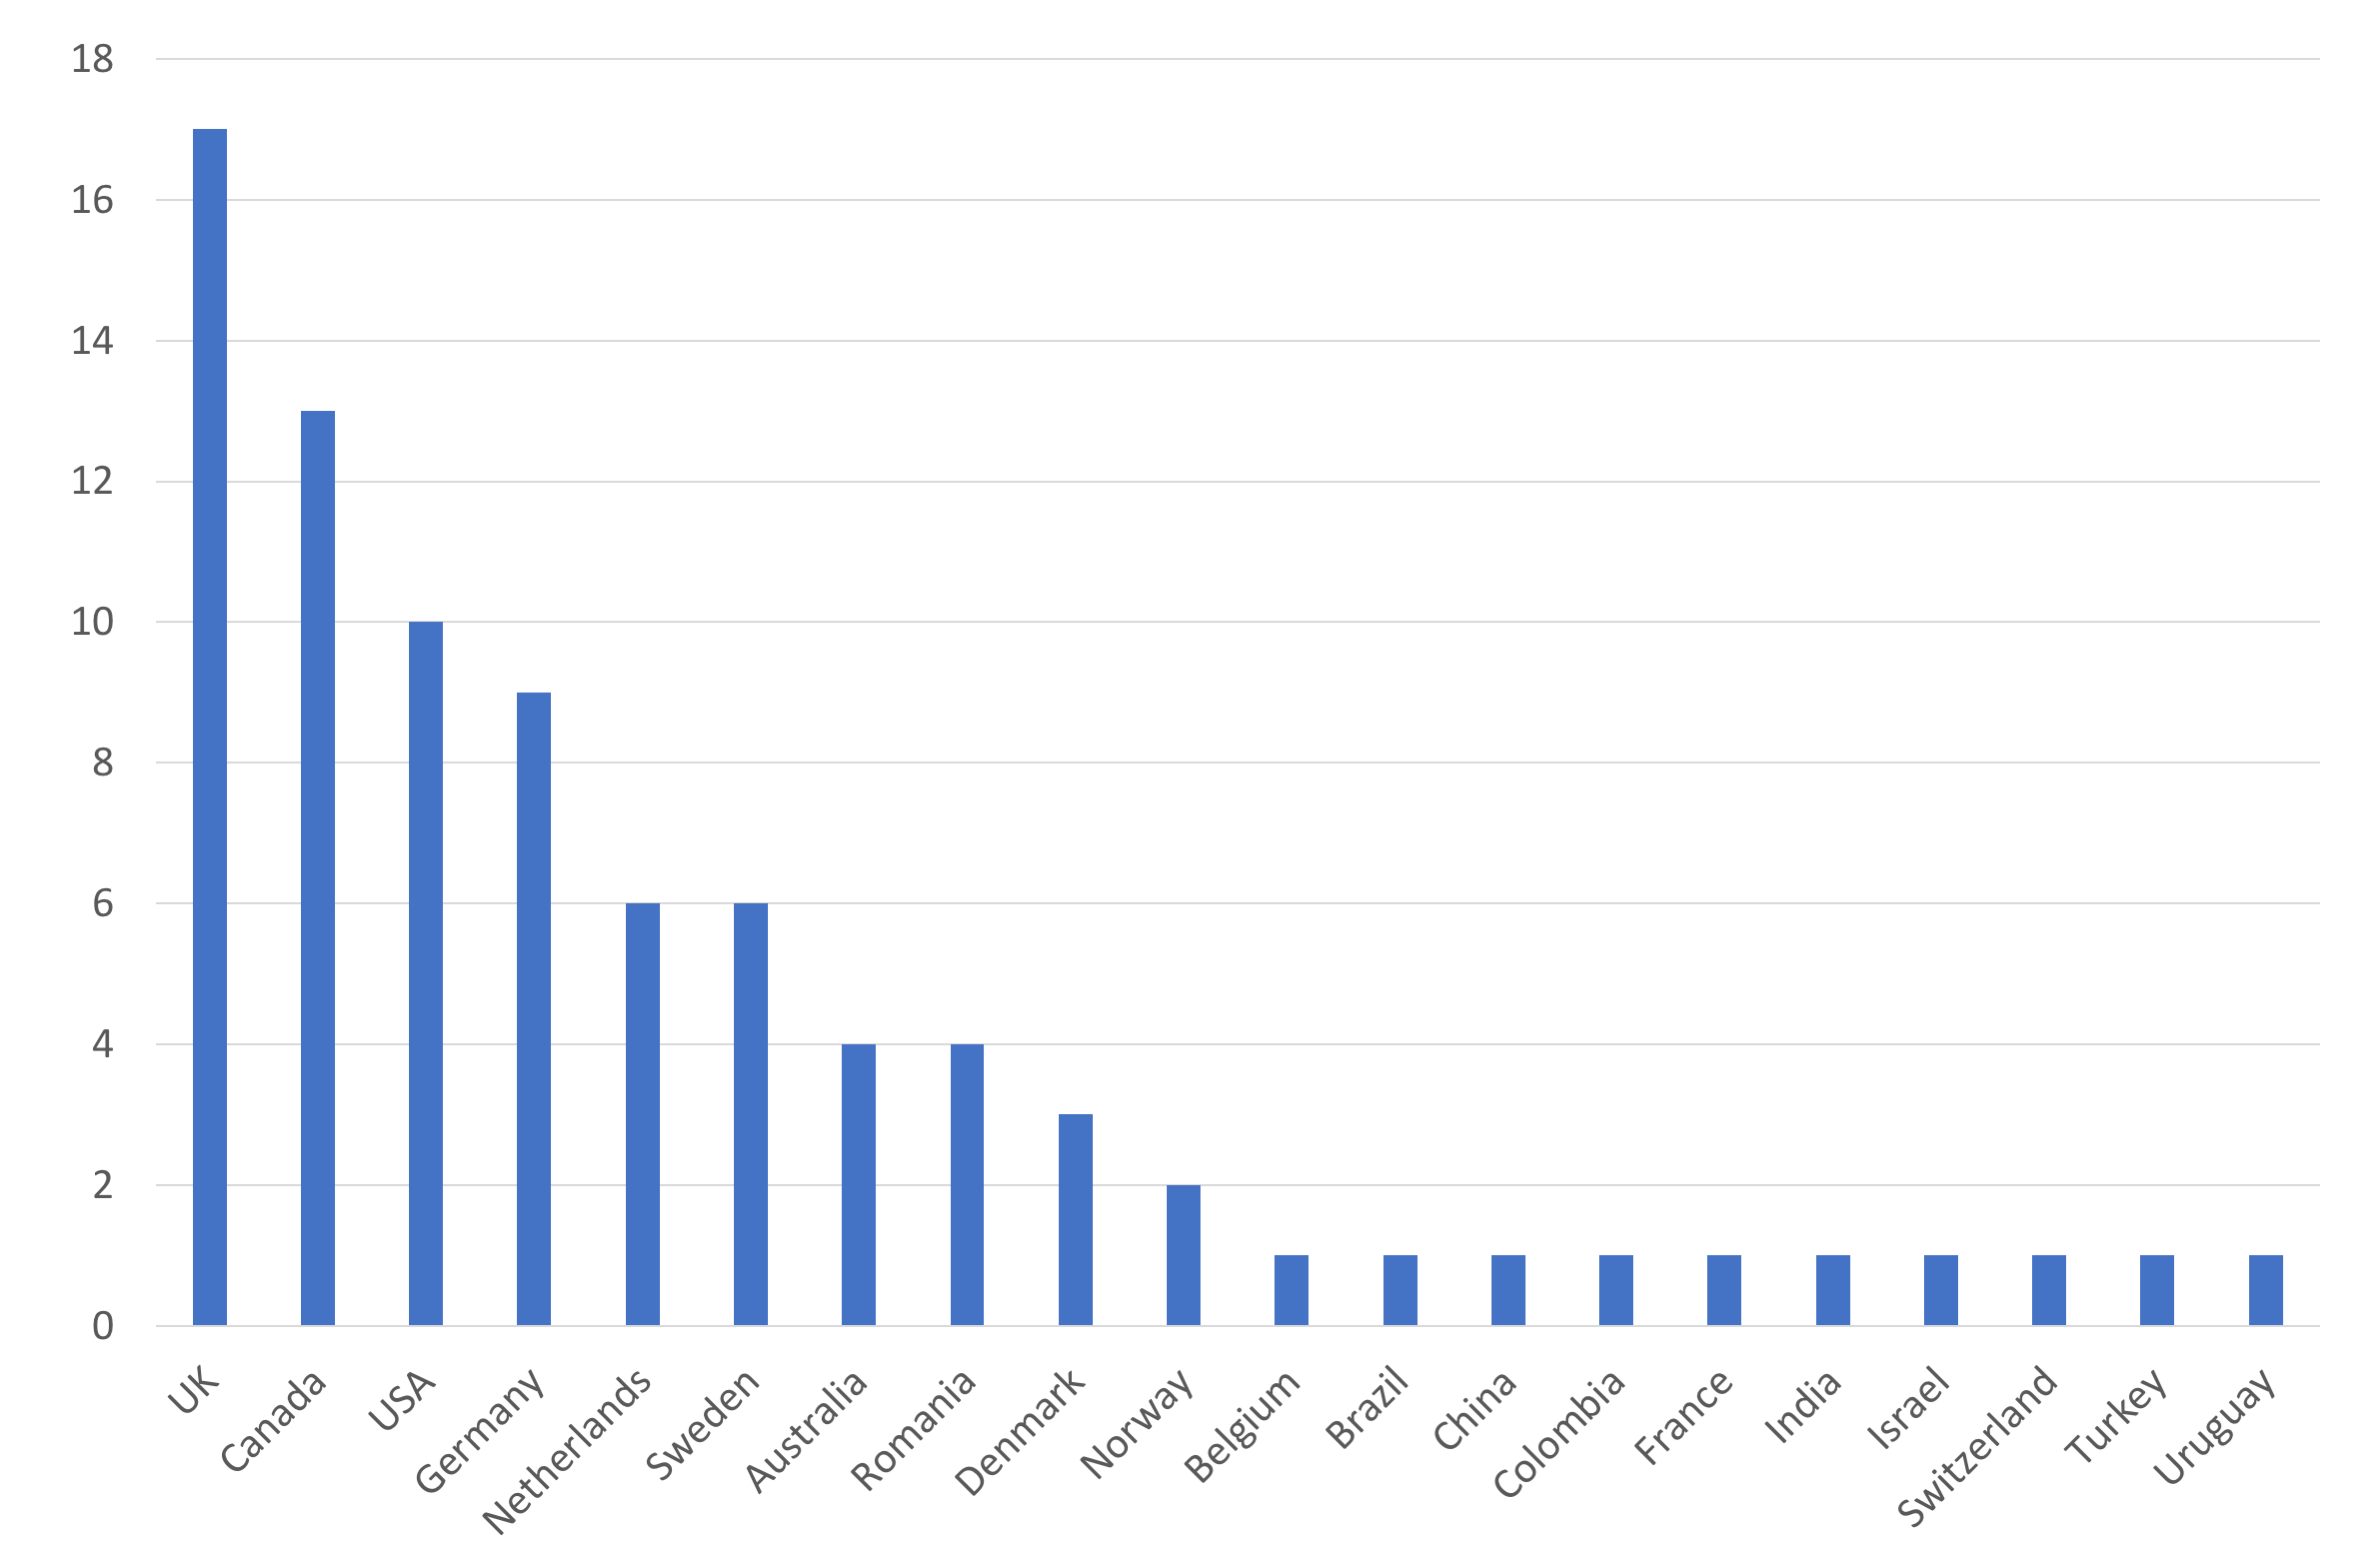
\includegraphics[width=12cm,trim={2 2 2 2},clip]{Figures/prioritisation-iplocation}
\caption{Respondent IP Address Locations}
\label{figure:iplocations}
\end{figure}

The result of using the respondents' IP address geographical locations to find which countries the questionnaire was completed form is shown in Figure \ref{figure:iplocations}.  While we must be cautious in assuming that these geographical locations are necessarily the locations of the respondents' homes and workplaces, it is a useful cross-check on the data.  We can see that 20 countries are represented, with 6 countries having 4 correspondents or more (which is roughly 5\% of the survey size).  These larger 6 countries are the UK, Canada, the USA, Germany, the Netherlands, Sweden, Australia and Romania.  Ten of the countries (Brasil, China, Columbia, France, India, Israel, Switzerland, Turkey and Uruguay) only had one survey completed from one of their IP addresses.  Just over 55\% of the responses were from IP addresses located in four countries, the UK (20\%), Canada (15\%), the USA (12\%) and Germany (11\%).

We discuss the possible impact of geographical location more when we consider threats to validity in section \ref{sec:threats}, but we think it is fair to say that we achieved good cross-geographic participation, but still ended up with a strong bias to Western Europe and North America.

The final classification we asked our respondents for was the number of years of experience that they had.  We asked this to ensure that participants had a significant amount of professional practice upon which to base their evaluation of the model and to allow us to understand if there are differences in the value of the model to architects with different amounts of experience.  The degree of experiences for our respondents is summarised in Figure \ref{figure:yearsexp}.
 
\begin{figure}
\centering
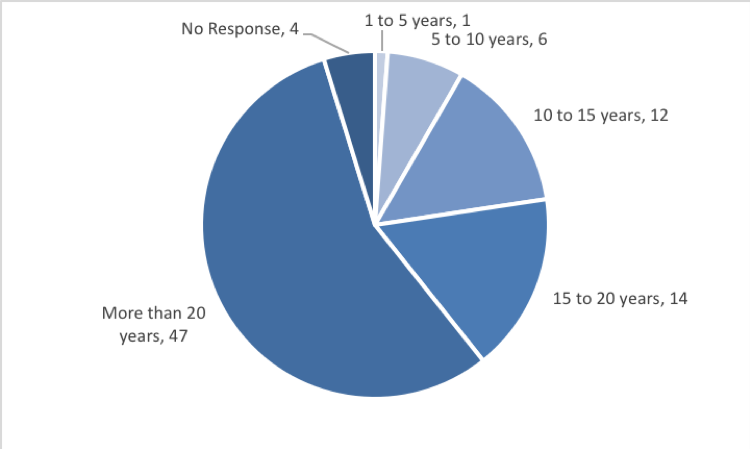
\includegraphics[width=8cm,trim={2 2 2 2},clip]{Figures/prioritisation-yearsexp-detailed}
\caption{Years of Experience of Respondents}
\label{figure:yearsexp}
\end{figure}

The obvious first impression is that our respondents were overwhelmingly experienced people, with over half of them (55\%) having at least 20 years of post-graduation experience.  At the other extreme only one respondent had less than 5 years of experience.  About 7\% had 5 to 10 years of experience, 15\% had 10 to 15 years and about 17\% had 15 to 20 years.  Four of our correspondents did not answer this question.

\subsection{The Results}

As mentioned earlier, we structured the questionnaire into two distinct parts, the closed-ended questions that asked people to rate the usefulness of the model and the open-ended questions that asked whether we had missed important risk areas to use with the prioritisation heuristic or whether there were any significant aspects of prioritisation that were completely missing from the model.

In this section, we review and analyse the responses to the closed-ended questions in the survey.
The first question we asked was to find out if the model was similar to how experienced architects already focused their attention, which would suggest that the model was credible and, if we assume that experienced architects are probably effective, a useful guide for less experienced architects, early in their career.  The responses we received from all of the respondents are summarised in Figure \ref{figure:similarity}.
 
\begin{figure}
\centering
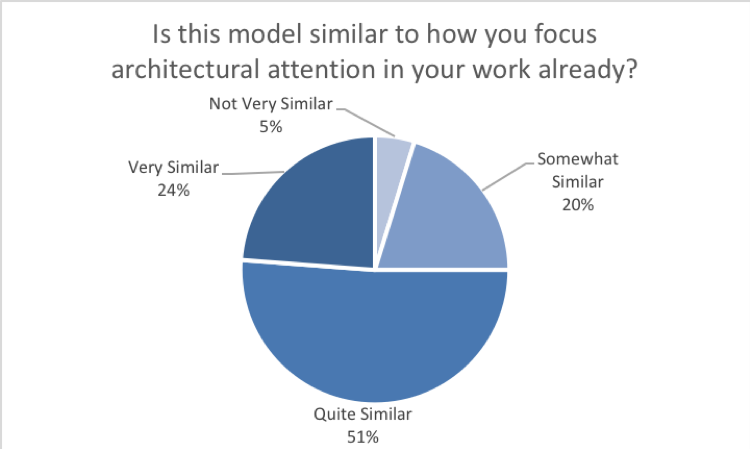
\includegraphics[width=8cm,trim={2 2 2 2},clip]{Figures/prioritisation-similarity}
\caption{How Similar the Model is to Existing Practice}
\label{figure:similarity}
\end{figure}

Considering all of the responses, the model validates quite strongly against the participants' existing practice, with 75\% of respondents stating that it was "very similar" or "quite similar" to their existing approach for focusing attention in their architecture work.  20\% said it was "somewhat similar", 5\% said it was not very similar to how they worked, and no respondents replied, "not at all similar".

Given that we were interested in attracting experienced architects to validate the model, we were also interested in finding out whether the number of years of experience altered their view of how similar the model was to how they worked.  The summary of this information is shown in Table \ref{table:similaritybyexp}.


\begin{table}
\caption{Similarity of the Model to Practice by Experience Level}
\label{table:similaritybyexp}
\footnotesize
% {l p{0.5cm} p{0.5cm} p{0.5cm} p{0.5cm} p{0.5cm} p{0.5cm} p{0.5cm} p{0.5cm} p{0.5cm} p{0.5cm}}
\begin{tabular}{l rrrrrrrrrr}
                & \multicolumn{2}{P{1.5cm}}{Not at All Similar} & \multicolumn{2}{P{1.5cm}}{Not Very Similar} & \multicolumn{2}{P{1.5cm}}{Somewhat Similar} & \multicolumn{2}{P{1.5cm}}{Quite Similar} & \multicolumn{2}{P{1.5cm}}{Very Similar} \\
1 to 5 Years       && &   &        &    &       & 1  & (100\%) &	&        \\
5 to 10 Years      && & 1 & (17\%) & 2  &(33\%) & 1  & (~17\%) & 2  & (33\%) \\
10 to 15 Years     && & 1 & (8\%)  & 3  &(25\%) & 7  & (~58\%) & 1  & (8\%)  \\
15 to 20 Years     && &   &        & 1  &(7\%)  & 11 & (~79\%) & 2  & (14\%) \\
More than 20 Years && & 2 & (4\%)  & 10 &(21\%) & 22 & (~47\%) & 13 & (28\%) \\
\end{tabular}
\end{table}

The table shows how many respondents, grouped by years of experience, rated the model at each similarity level, compared to their own approach to prioritising their work.  The 4 participants who did not indicate their experience level are excluded from this table.  The percentage values are the percentage of the participants in the current row that the value represents.

We are primarily interested in the top three groups, which is architects with at least 10 years of experience.  What we can see from this data is that the degree of similarity between the model and the architect's current practice does vary between these three groups, with 66\% of the 10 - 15 year group rating it as "quite similar" or "very similar", 93\% of the 15 - 20 years group rating it at this level and 75\% of the 20+ year group rating it in this way.  So, all three groups validate quite strongly, but it seems to reflect most strongly how the 15+ year groups work.

The second question moved on to try to establish, whether the respondents thought that the model would be useful in practice.  A summary of the answers to this question across all responses is shown in Figure \ref{figure:helpfulness}.
 
\begin{figure}[h]
\centering
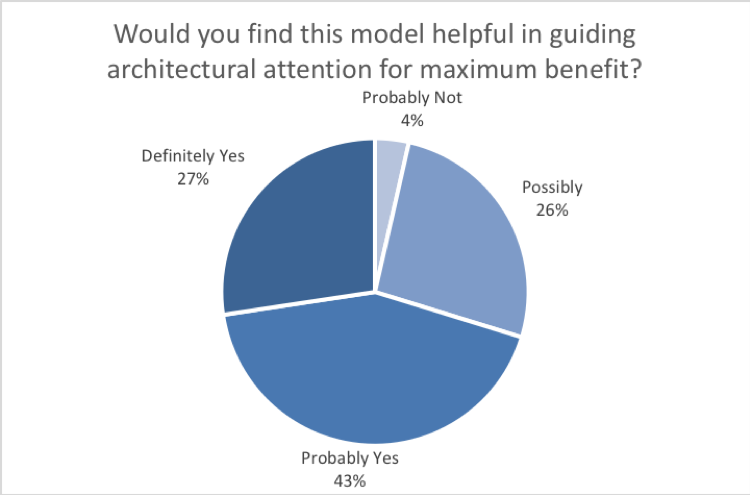
\includegraphics[width=8cm,trim={2 2 2 2},clip]{Figures/prioritisation-helpfulness}
\caption{Helpfulness of the Model}
\label{figure:helpfulness}
\end{figure}

Across all of the respondents, 70\% said that it was definitely or probably useful, which we interpret as a strong overall validation of the model.  The remaining respondents mainly stated that they might "possibly" find it useful.  Only 3 respondents said "probably not" and none said, "definitely not".
We were interested in how the utility of the model might vary by the experience of the respondent, so we performed a similar analysis by experience group to that performed for the previous question.  The results are shown in Table \ref{table:helpfulness}.

\begin{table}
\caption{Helpfulness of the Model by Experience Level}
\label{table:helpfulness}
\footnotesize
\begin{tabular}{l P{1.5cm} P{1.5cm} P{1.5cm} P{1.5cm} P{1.5cm}}
 & Definitely Not & Probably Not & Possibly & Probably Yes & Definitely Yes \\
1 to 5 Years       & &          &           &           & 1 (100\%) \\
5 to 10 Years      & & 1 (17\%) & 3 (50\%)  & 2 (33\%)  & \\
10 to 15 Years	   & &          & 4 (33\%)  & 5 (42\%)  & 3 (25\%) \\
15 to 20 Years     & &          & 4 (29\%)  & 5 (36\%)  & 5 (36\%) \\
More than 20 Years & & 2 (~4\%)  & 10 (26\%) & 23 (43\%) & 12 (26\%) \\
\end{tabular}
\end{table}

Again, focusing on the architects with at least 10 years of experience, 67\% of the 10 to 15 year experience group believe the model is "probably" or "definitely" useful, 72\% of the 15 to 20 year group also rate it at this level, while 69\% of the most experienced, 20+ years of experience group, believe it is "probably" or "definitely" useful.  A strong majority of respondents in all three groups appear to find the model useful, with the strongest validation coming from the 15 - 20 years of experience group.

Finally, we wanted to check that the areas of risk we had identified as important within the "prioritise time according to risks" heuristic were valuable to a practising architect.  The results of the corresponding question in the survey across all respondents are shown in Figure \ref{figure:validationofareas}.

\begin{figure}[h]
\centering
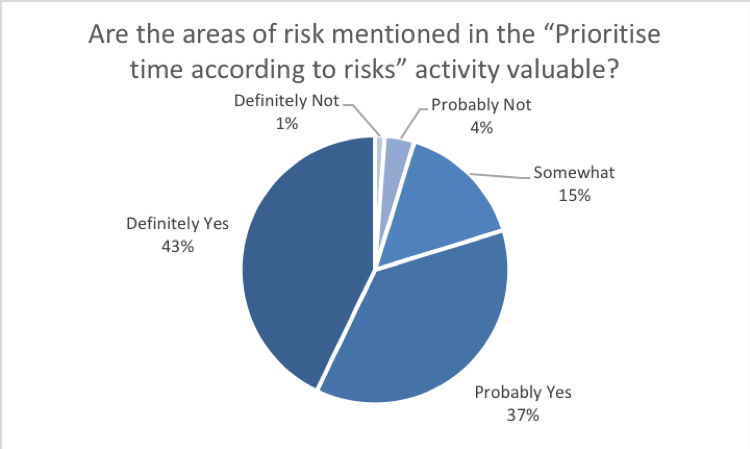
\includegraphics[width=8cm,trim={2 2 2 2},clip]{Figures/prioritisation-riskareas}
\caption{Validation of Risk Prioritisation Areas}
\label{figure:validationofareas}
\end{figure}

In this case we did have one very strong negative opinion ("definitely not") but this was a single individual (an enterprise architect in the 10 - 15 years of experience group, who commented in the open-ended questions that he did not believe that it was possible to define general software development risks in a useful way).

Beyond this response, 80\% of respondents believe that the areas of risk were "definitely" or "probably" valuable, suggesting that this aspect of the model should be of value to many practitioners.

Again, we analysed the responses by the experience level of the respondent, which is shown in Table \ref{table:valueofriskfactors}.

\begin{table}
\caption{Value of Risk Factors by Experience Level}
\label{table:valueofriskfactors}
\footnotesize
\begin{tabular}{l P{1.5cm} P{1.5cm} P{1.5cm} P{1.5cm} P{1.5cm}}
 & Definitely Not & Probably Not & Somewhat & Probably Yes & Definitely Yes \\
1 to 5 Years       &         &          &          &           & 1 (100\%) \\
5 to 10 Years      &         & 1 (17\%) & 1 (17\%) & 2 (33\%)  & 2 (~33\%) \\
10 to 15 Years     & 1 (8\%) &          &          & 5 (42\%)  & 6 (~50\%) \\
15 to 20 Years     &         &          & 3 (21\%) & 6 (43\%)  & 5 (~36\%) \\
More than 20 Years &         & 2 (4\%)  & 9 (19\%) & 17 (36\%) & 19 (40\%) \\
\end{tabular}
\end{table}


Looking at the architects with more than 10 years experience, we still see a high degree of validation (92\% of 10 to 15 year experience respondents, 79\% of 15 to 20 year respondents and 76\% of respondents with more than 20 years of experience saying "probably yes" or "definitely yes") but there is a larger range of opinion than before.

We had the single individual who strongly disagreed with the risk factors being valuable in the 10 - 15 year group, 3 respondents in the 15 to 20 years of experience group only feeling that they were "somewhat" valuable and 11 respondents with more than 20 years of experience stating that the factors were "somewhat" or "probably not" valuable.

This said, we still feel that the degree of validation that the model received across all of the experience levels indicates that the model has a high possibility of being useful to at least a majority of practitioners.

We were also interested to investigate if the key question of how useful the model was would vary significantly between our different respondent groups, particularly by job family and geography, which might suggest that the model aligned better with certain types of architecture work or practice in certain parts of the world.

We have analysed the responses to the question "Would you find this model helpful in guiding architectural attention for maximum benefit?" by role type and the results are shown in Table \ref{table:usefulnessbyrole} and Figure \ref{figure:usefulnessbyrole}.

\begin{table}
\caption{Usefulness of the Model by Role Type}
\label{table:usefulnessbyrole}
\footnotesize
\begin{tabular}{l P{1.5cm} P{1.5cm} P{1.5cm} P{1.5cm} P{1.5cm}}
 & Definitely Not & Probably Not & Possibly & Probably Yes & Definitely Yes \\
Software Architect	 &  &  1 (~3\%) & 11 (35\%)  & 13 (42\%) & 6 (19\%) \\
Software Designer    &  &  1 (10\%) &  ~2 (20\%) & ~5 (50\%) & 2 (20\%) \\
Solution Architect   &  &           &  ~2 (25\%) & ~5 (63\%) & 1 (12\%) \\
Technical Architect	 &  &           &            & ~2 (50\%) & 2 (50\%) \\
Enterprise Architect &  & 1 (~4\%)  & ~4 (17\%)  & ~9 (39\%) & 9 (39\%) \\
\end{tabular}
\end{table}

\begin{figure}[h]
\centering
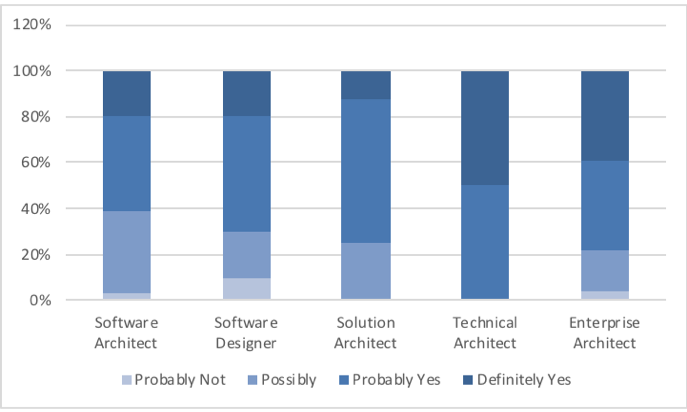
\includegraphics[width=8cm,trim={2 2 2 2},clip]{Figures/prioritisation-usefulness-by-role}
\caption{Usefulness of the Model by Role Type}
\label{figure:usefulnessbyrole}
\end{figure}

As can be seen, all of the respondent role groups validated the model as "probably" or "definitely" useful, with the lowest validation (interestingly) coming from the Software Architect group, where 61\% of the respondents indicated this level of agreement (although nearly all of the remaining respondents were neutral - "possibly" - rather than negative).  In the Software Designer group 70\% of respondents, in the Solution Architect group 75\%, in the Technical Architect group 100\% and in the Enterprise Architect group 78\% of respondents considered the model to be "definitely" or "probably" useful.

Turning to the possible influence of geographical location, we analysed the same question as to the usefulness of the model by the respondents, by the geographical location that the respondents told us they were from.  The results are summarized in Table \ref{table:usefulnessbygeo} and Figure \ref{figure:usefulnessbygeo}.

\begin{table}
\caption{Usefulness of the Model by Geography}
\label{table:usefulnessbygeo}
\footnotesize
\begin{tabular}{l p{1.5cm} p{1.5cm} p{1.5cm} p{1.5cm} p{1.5cm}}
% slightly experimental bit here - aligns headers centrally and leaves the
% others with default alignment from the definition above
% https://tex.stackexchange.com/questions/2924/how-to-align-table-headers-differently-than-all-other-table-cells
 & \centering Definitely Not & 
   \centering Probably Not & 
   \centering Possibly & 
   \centering Probably Yes & 
   \centering Definitely Yes \tabularnewline
Americas              & &         & ~6 (23\%)  & 10 (38\%) & 10 (38\%) \\
Asia-Pacific          & &         & ~3 (50\%)  & ~3 (50\%) & \\
Europe (inc. UK)      & & 3 (6\%) & 11 (23\%)  & 22 (45\%) & 11 (23\%) \\
Middle-East \& Africa & &         & ~1 (100\%) &           & \\
\end{tabular}
\end{table}
 
\begin{figure}
\centering
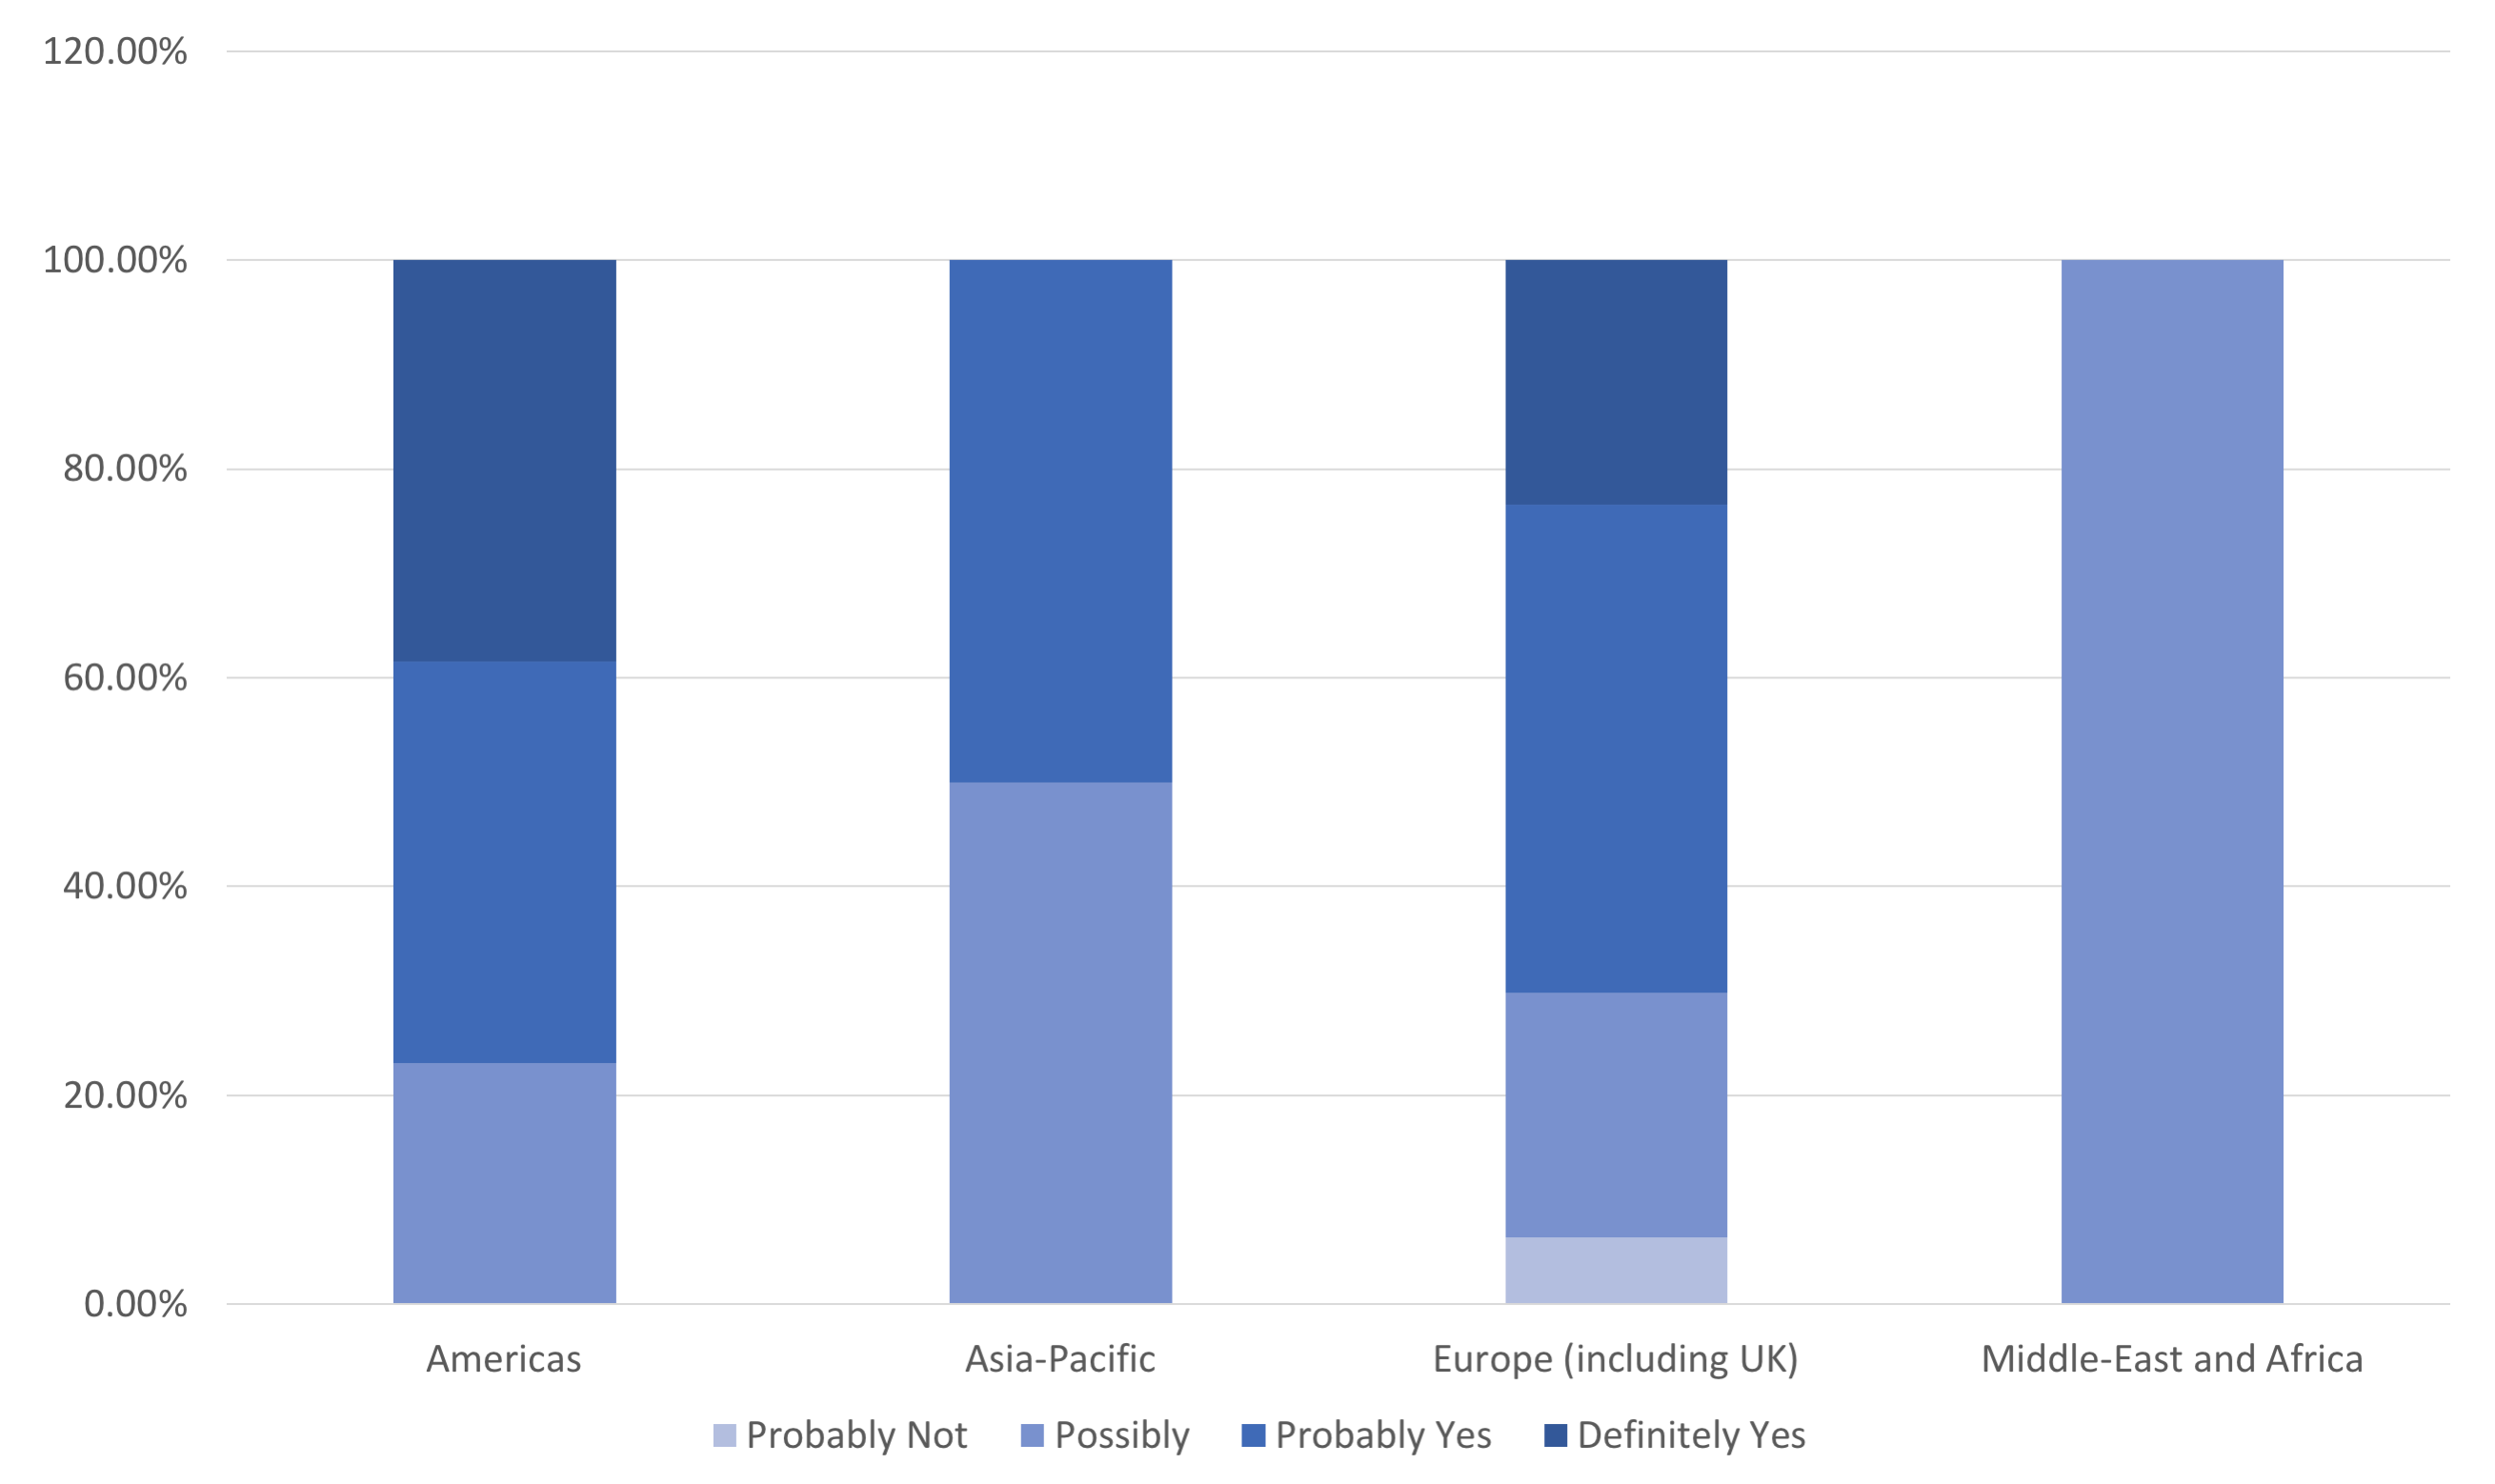
\includegraphics[width=8cm,trim={2 2 2 2},clip]{Figures/prioritisation-usefulness-by-geo}
\caption{Usefulness of the Model by Geography}
\label{figure:usefulnessbygeo}
\end{figure}

In this analysis, we have included all of the regions, but in reality, the data for the Middle-East and Africa and Asia-Pacific is difficult to use with confidence as there were very few respondents from these regions (1 from ME\&A and 6 from APAC).  Therefore, while recognising the importance of these regions and their contribution to contemporary software engineering, we focus on Europe and the Americas for the purposes of this specific analysis.

We had 26 respondents from the Americas and 69 from Europe (including the UK).  Both of these contributions are large enough to be significant, being 31\% and 82\% of the total responses, respectively.

Of these significant geographical groups, the group from the Americas validated the usefulness of the model more strongly, with 76\% of respondents indicating that the model was "definitely" or "probably" useful.  For the European group, 68\% of the respondents indicated that the model was "definitely" or "probably" useful.

We interpret this data as suggesting that the model validates well in both the Americas and in Europe and should be useful in both regions.  The data we have suggests that it should also be useful in Asia-Pacific as 50\% of respondents indicated it would be useful, while in contrast, it may not be useful in ME\&A as our single respondent from that region indicated it was "probably not" useful; However, we do not have enough respondents from these regions to draw meaningful conclusions.  To investigate the usefulness of the model in APAC and the Middle-East and Africa would require a further study.

In summary, having analysed the answers to the closed-ended answers in our survey, we conclude that our model is likely to be credible and useful in Europe and the Americas and broadly aligns with the prioritisation approach used by many experienced architects in those regions.
We view this as a successful validation of the model; However, we were also interested in how the model could be improved and so we used the responses to the open-ended questions in the survey to find themes which we could include in a refined model.

\subsection{Analysing the Open-Ended Responses}
\label{sec:openended}

As explained earlier, we asked two important open-ended, questions, Q4, to identify missing risk factors from the "prioritise time according to risks" heuristic ("are there other general areas of risk that should be added to "prioritise time according to risks" that would be applicable to most (information) systems and environments?") and Q5, to ask whether we had missed any important aspect of the model entirely ("are there any significant factors missing from the model which you use to focus your architectural work?").

We had 44 responses to Q4, about missing aspects of the model, and 51 responses to Q5, about missing areas of risk.

Given the nature of these responses, we again used grounded theory style analysis to analyse them, coding each one initially using straightforward, descriptive labels, directly reflecting the language used in the response, then refining this with further coding steps, to identify higher-level categories to allow the responses to be collected into meaningful groups.

For the first question, Q4, we initially coded the responses to 37 distinct categories, plus two null categories for the initial coding of "None" and "General Comment" for those responses which were present but did not specify a new risk area or just made a general comment.  The responses suggested a diverse range of possible risk areas, and when we refined the coding to find common concepts, this resulted in 24 higher level categories.  We attempted to refine this further but did not find further meaningful refinements as we tried further rounds of coding (we judged that we had reached "theoretical saturation" with the data).   In addition, we had a very long "tail" of concepts with only a single mention in the responses, leaving us with 5 categories that had 4 responses or more: Organisational Environment (11 occurrences), Stakeholders (6 occurrences), Cost (6 occurrences), Time (4 occurrences), External Environment (4 occurrences).  We chose to focus on categories with at least 4 occurrences as this represents approximately 5\% of the total respondents to the survey and we judged this to be high enough to warrant consideration.

In the context of a survey with over 80 responses, none of the categories of response for missing risk factors was universally viewed as important, but we felt that it was important to reflect the fact that these four factors had been independently identified by a number of people.  Therefore, we decided to integrate these new factors into the refined version of the model.

For the second open-ended question, Q5, on missing aspects of the model, we initially coded the responses into 43 distinct categories, again plus "None" and "General Comment".  As we continued with the process of refining the coding further, we ended up with 26 higher level categories.  As with the responses to Q4, many of the categories were only mentioned once and only four were mentioned 4 times or more: Team Effectiveness (10), Benefits (7), Stakeholders (6) and Time (5).  Of these factors, "Stakeholders" are already a significant factor in the model and the comments provided in these cases were suggesting a particular emphasis on certain stakeholders or method of dealing with stakeholders.  The specific suggestions were all different and stakeholder needs and priorities are already a significant part of the model, so we did not feel that a new model element was needed, but we simply need to review the detailed comments and ensure that they are reflected in the existing elements of the model.

In this context, we felt that adding a completely new aspect to the model was a significant step and so we only wanted to consider this for aspects which had been identified as important by a significant number of respondents to the survey.  On this basis, we decided to add a new element to the model to reflect the "Team Effectiveness" theme as it was the only additional candidate aspect that at least 10\% of the respondents had identified as important.

Finally, we also received 37 general comments in the open-ended question at the end of the survey along with another 14 responses to the other open-ended questions which we judged to be general comments rather than specific answers to those earlier questions, making a total of 51 general comments.  We do not view these responses as part of the validation of the model, but some of them did provide useful commentary on the work.  Again, we used a grounded theory style coding approach to analyse the data and this resulted in 23 categories of comment.  Like the other open-ended questions, most of these categories were not judged as significant because less than four respondents mentioned them.

The categories which had four or more respondents were general Positive Comments such as "nice and simple model" (14), comments on the How the Architect Should Work, such as "an architect must help implement what he/she helped to decide" (6) and comments on the Presentation of the Model, such as "this model [\ldots] does appear to be a rather linear, and distinct,  in reality it [the process] is quiet iterative and overlapping" (sic) (5).

We found all of the general comments interesting and potentially useful, but most of them did not lead us to conclude that further changes were needed to the model.  The exception was the group of comments categorised as Presentation of the Model.  These 5 comments suggested that the respondents interpreted our graphical presentation of the model as indicating a linear "upfront" process.  In fact, we had meant to communicate exactly the opposite through our diagram, and indicate that the process is iterative and continuous, happening right through the project's lifecycle.  We took this as an important indicator that we needed to change the graphical representation of the model and also describe its intended iterative and continuous nature more clearly in the supporting text.

\section{Stage 4 - Refined Model for Prioritising Architectural Effort}
\label{sec:refined-model}

We took the outputs of the open-ended question analysis described in section \ref{sec:openended} and used them to add missing features of the model, improve the list of risks to suggest for time prioritisation and improve the model using the advice provided in the general comment responses to the survey.
The result of these additions is a refined model for prioritising architectural effort, with an additional feature of the model, "Team Effectiveness" and a refined list of risks for time prioritisation.  As mentioned earlier, we also decided to alter the graphical presentation of the model to try to emphasise that it is not a linear "process" but rather a set of activities to be performed throughout the project lifecycle.  The refined model is shown in Figure \ref{figure:refinedmodel}.

\begin{figure}
\centering
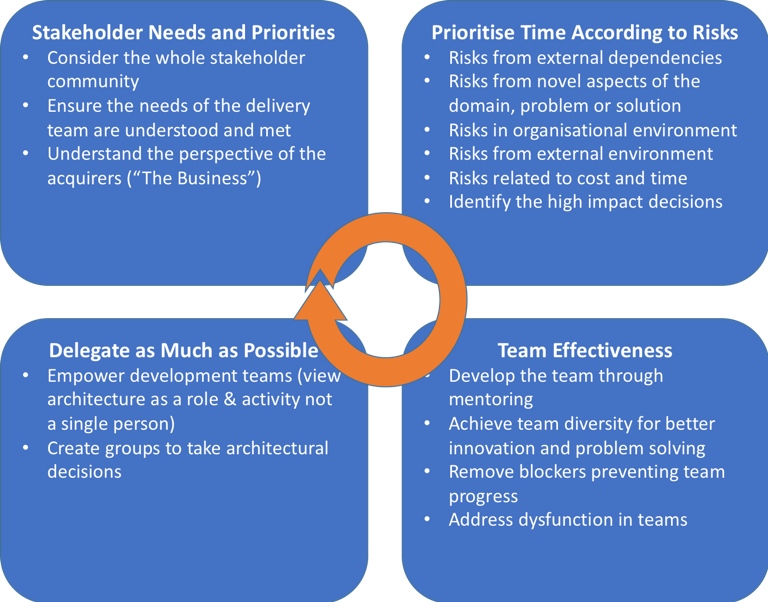
\includegraphics[width=12cm]{Figures/prioritisation-refined-model}
\caption{Refined Model for Prioritising Architectural Attention}
\label{figure:refinedmodel}
\end{figure}

The model is comprised of 4 aspects, Stakeholder Needs and Priorities, Prioritise Time According to Risks, Delegate as Much as Possible and Team Effectiveness.  Each aspect is a theme which our initial interviewees and the later survey respondents find useful when considering how to prioritise their architectural work.  The details of each theme are described in the subsections below. 

The idea of the model is to provide a guide for new architects, or an aide-memoir for experienced architects, on how to prioritise their architectural work in order to maximise its effectiveness.  It is not a process or a step to be followed in an architectural "method" but rather these are themes for effective effort prioritisation that should be repeatedly considered during the lifecycle of a project.
As with any set of heuristics, they can only be a generalised starting point and need to be considered, interpreted and applied in a context-specific way by the architects and teams who use them.  However, they have validated well against a reasonably broad survey of experienced, practising architects and so we believe that they are a useful starting point upon which to build a personal approach for prioritisation.

\subsection{Stakeholder Needs and Priorities}

The first theme which emerged strongly in our study was focusing on the needs and priorities of the stakeholders involved in the situation.  The principle that architecture work involves working closely with stakeholders is widely agreed \cite{rozanski2011-ssa2e, bass2012-sainp}, and this theme reinforces that. Architects need to focus significant effort to make sure that stakeholder needs and priorities are understood to maximise focus on the critical success factors for a project and maximise the chances of its success.  Three specific heuristics to achieve this which emerged from the study are:

\begin{itemize}
	\item \emph{Consider the whole stakeholder community}. Spend time understanding the different groups in the stakeholder community and avoid the mistake of just considering obvious stakeholder groups like end-users, acquirers and the development team.  As the architecture methods referenced above note, ignoring important stakeholders (like operational staff or auditors) can prevent the project from meeting its goals and cause significant problems on the path to production operation.
	\item \emph{Ensure that the needs of the delivery team are understood and met}.  Spend sufficient time to ensure that the delivery team can be effective.  What is the team good at?  What does it know?  What does it not know?  What skill and knowledge gaps does it have?  These areas need attention early in the project so that architecture work avoids risks caused by the capabilities of the team and that time is taken to support and develop the team to address significant weaknesses.
	\item \emph{Understand the perspective and perceptions of the acquirers of the system}.  Acquirers are a key stakeholder group who judge its success and usually have strategic and budgetary control, so can halt the project before delivery if they are unhappy.  Specifically addressing this group's needs, perceptions and concerns emerged as an important factor for some of the experienced architects in our study.  Acquirers are often senior managers and so may be distant from the day-to-day reality of a project and need regular, targeted, clear communication to understand their concerns and ensure that they have a realistic view of the project. 
\end{itemize}

\subsection{Prioritise Effort According to Risks}

During a project, an effective approach to prioritising architectural attention is to use a risk-driven approach to identify the most important tasks.  If the significant risks are understood and mitigated, then enough architecture work has probably been completed.  If significant risks are open, then more architecture work is needed. The specific heuristics to consider for risk assessment are:

\begin{description}
	\item \emph{Risks from external dependencies}.  Understand your external dependencies because you have little control over them and they need architectural attention early in the project and whenever things change.
	\item \emph{Risks from novel aspects of the domain, problem or solution}.  Another useful heuristic, from the experience of our study participants, is to focus on novelty in your project.  What is unfamiliar?  What problems have you not solved before?  Which technology is unproven? The answers to these questions highlight risks and the participants in our study used them to direct their effort to the most important risks to address.
	\item \emph{Risks in the organisational environment}.  Each organisation is different and there are nearly always risks specific to an environment such as the internal political situation, what is possible in the organisational culture, and the maturity of the organisation with respect to architecture, change and risk.  Different organisations also have different cultures and capabilities for funding change, which can create risks.  The speed which different sorts of risk and difficulties can be addressed can also be affected by organisational factors and so may cause you to change where you focus attention.  Participants in our study noted the importance of "situational awareness" \cite{wikipedia-sitawareness} that allows the architect to find and address the risks specific to their organisational environment.
	Risks from the external environment.  Nearly all organisations exist in a complex ecosystem of interacting partners, customers regulators, competitors and other actors and they can be a source of risk for many systems, as can general trends and changes in the industry that the organisation exists within (such as changing regulatory environment or industry-wide pressures such as reducing margins on products or services). 
	\item \emph{Risks related to cost and time}.  Most architects will report that they are often expected to achieve challenging goals in unrealistic timescales or with unrealistic cost estimations.  Many of our study participants reported that they needed to focus significant attention on risks resulting from cost and time.
	\item \emph{Identify the high impact decisions}.  Prioritise architecture work that will help to mitigate risks where many people would be affected by a problem (e.g. problems with the development environment or problems that will prevent effective operation) or where the risk could endanger the programme (e.g. missing regulatory constraints).
\end{description}

\subsection{Delegate as Much as Possible}

Delegation was an unexpected theme that emerged from our study. The architects who mentioned this theme viewed themselves as a potential bottleneck in a project and delegation and empowerment of others was a way to minimise this.  Delegation was also seen as a way of freeing the architect to focus on the aspects of the project that they had to focus on rather than all the other aspects that they could possibly get involved in.

The general message of this theme is to delegate as much architecture work as possible to the person or group best suited to perform it, to prevent individuals becoming project bottlenecks, allow architects to spend more time on risk identification and mitigation, and to spread architectural knowledge through the organisation.  The heuristics that were identified to help achieve this are:

\begin{description}
	\item \emph{Empower the development teams}. To allow delegation and work sharing, architects need to empower (and trust) the teams that they work with.  This allows governance to become a shared responsibility and architecture to be viewed as an activity rather than something that is only performed by one person or a small group.  This causes architectural knowledge, effort and accountability to be spread across the organisation, creates shared ownership, reduces the load on any one individual and prevents reliance on a single individual from delaying progress.
	\item \emph{Create groups to take architectural responsibilities}.  A related heuristic is to formalise delegation somewhat and create groups of people to be accountable for specific aspects of architectural work.  For example, in a large development programme, an architecture review board can be created to review and approve significant architectural decisions.  Such a group can involve a wide range of expertise from across the programme and beyond, so freeing a lead architect from much of the effort involved in gathering and understanding the details of key decisions, while maintaining effective oversight to allow risks to be controlled and technical coherence maintained.  Similarly, a specific group of individuals could be responsible for resilience and disaster recovery for a large programme, allowing them to specialise and focus on this complex area, and allowing a lead architect to confidently delegate to them, knowing that they will have the focus and expertise to address this aspect of the architecture.
\end{description}

\subsection{Team Effectiveness}

A theme that emerged when we validated our initial model with a wider group was the need to focus attention on making sure that the overall development team was as effective as possible.  The participants who indicated the importance of this factor were concerned with the need to develop the individuals in the team and to ensure that the team was as diverse as possible, to allow it to use a range of skills and perspectives when innovating and solving problems.

Other aspects of this theme that participants were concerned with were the importance of architecture work being used to quickly unblock the team when it hit difficulties and the importance of technical leaders, like the architect, to step in when needed to make sure that the team was functioning well and to address any dysfunctional behaviour observed.

The heuristics that the participants identified as being important for focusing architectural attention to achieve team effectiveness were:
\begin{description}
	\item \emph{Develop the team through mentoring}.  Every team should be on a collective journey towards improvement and hopefully, every individual in a team is on a similar personal journey to be the best that they can be.  People doing architecture work tend to be some of the most experienced people in a team and so a valuable and important area to focus attention, in order to achieve a highly effective team, is to spend time developing the individuals in the team, and the team as a whole, through thoughtful, intentional mentoring.
	\item \emph{Achieve team diversity for better innovation and problem-solving}.  In order to innovate and identify good solutions to problems, it is valuable to have a range of experience, perspectives and skills in the team.  Our study participants indicated that a valuable use of architectural time is to spend time building diverse teams that can achieve this.
	\item \emph{Remove blockers preventing team progress}.  Development and support teams often tend up blocked by technical or organisational factors, so spending time resolving these problems is a valuable focus for many architects.
	\item \emph{Address dysfunction in teams}.  Sometimes teams do not work well and it requires someone who is close to the team and respected by them, but outside the team structure, to identify the problem and suggest solutions.  Some architects work directly in individual teams and are not well placed to do this, but people doing architecture work are often close to the teams but outside their structure, and have the respect, soft-skills and experience to resolve team problems.  This use of architectural time can have huge benefits when dysfunctional behaviour is observed in teams.
\end{description}

\section{Threats to Validity}
\label{sec:threats}

We designed and conducted this study carefully to provide us with a useful model and a reliable evaluation of it, avoiding bias as much as possible.  Specific steps we took to produce a reliable evaluation of the model included focusing on the practitioner community (as they are the intended users of the model), focusing on experienced respondents who have the experience to evaluate the model, finding a reasonably large, geographically distributed group to validate it for us, structuring the questionnaire to allow disagreement as well as confirmation, and analysing the results in a careful, structured manner to allow the data to lead us to the conclusions, to avoid the danger of us subconsciously using it to validate an opinion we already held.  However, we acknowledge that there are potential limitations to any qualitative study, including ours, which can result in threats to our study's validity.

There are four main types of threat to the validity of a study like this, namely construct, internal, 
external and conclusion validity as defined in \cite{matt1994-threatstovalidity}. 

Construct validity is concerned with the relationship between theory and observation.  A commonly recurring threat when using questionnaires is the phrasing of the text, the questions and the responses to the closed-ended questions.  A second threat is where too many closed-ended questions are used and respondents cannot find suitable responses in the available set.  We addressed potential problems with wording by keeping the amount of text in the questionnaire as small as possible and using simple language that directly referenced the model.  The model itself was derived from the language and concepts that emerged from the semi-structured interviews.  We also tested the questionnaire ourselves and on a small number of other architects that we knew, to ensure that their interpretation of the questionnaire was as we expected and we refined the language slightly as a result.  We mitigated the possible problem of participants being unable to express their opinions through the closed-ended questions by limiting the closed-ended questions to being simple ratings and then providing open-ended questions for the participants to explain, expand or clarify their answers.

Internal validity is concerned with the validity of the causality relationship between the observations and the outcomes of the study.  We addressed this by using very straightforward analysis approaches, both for the statistical data analysis and for the analysis of open-ended answers, so the threats to the correctness of the analysis we performed are minor.  We also reviewed all of the answers from each respondent to ensure that they formed a credible and consistent set (which all did), so validating that the respondents understood the process and were expressing a coherent opinion.  To avoid possible misunderstanding we provided a clear definition of the model, links to additional information, trialled the questionnaire with people we knew, and included open-ended questions to allow respondents to express opinions that could not be easily captured using the closed-ended questions.

External validity is concerned with the generalisability of the results of the study.  The key risk we identified relating to external validity is an unrepresentative respondent population or a respondent population who lack competence in software architecture and so cannot validate the model effectively.  We mitigated these risks by finding a relatively large respondent population, who are distributed geographically, although as noted earlier, nearly all of the respondents came from Europe and the Americas.  So a residual risk we continue to have is the lack of representation from Asia, in particular, countries like India, China and Singapore, with significant software engineering populations and the potential for significant cultural differences from Europe and the Americas.  We mitigated the concerns around experience and competence by targeting experienced architects and architects in our extended professional network, whom we knew to be experienced and highly competent.  We know a significant percentage of the respondents at least slightly and through some informal sampling of employing organisations and job titles, have a high degree of confidence in the ability of our study participants to validate or critique the model correctly.  This leaves us with a residual risk that our extended network may be more likely to think similarly than a truly random sample, but anecdotally we do not believe that they are significantly different to most practitioners we have met over the years and we believe this trade-off to ensure credible study participants is the correct one.

Conclusion validity is concerned with the validity of the relationship between the data obtained in the study and the conclusions that have been drawn from it.  The threats that we identified in this area are whether we asked the right questions at each stage of the study, whether we made mistakes in analysing the data, and whether we introduced unconscious bias into the study which could invalidate our conclusions.  We mitigated the possibility of asking the wrong questions by using a semi-structured interview in the first stage and providing extensive opportunity for open-ended responses in the third stage.  We acknowledge that we could have made mistakes in our analysis and processing of the data, but we mitigated this by reviewing and cross-checking our work and using a simple, repeatable process which was straightforward to follow.  The largest risk to conclusion validity is probably the chance of introducing unconscious bias, as much of the study involved interpreting open-ended responses from the interviews and the questionnaire.  We attempted to mitigate this risk through the use of the grounded theory process, which helped us to be led by the data rather than trying to fit the data into a pre-existing theory.  We also reviewed our conclusions several times and repeated parts of the analysis if we felt that there was any danger of an alternative outcome being more representative.  We also did not have any preconceived ideas about the likely outcome of this study at the beginning, so did not have an underlying theory we were trying to validate.  Overall, we do not feel that we have been likely to introduce unconscious bias in the study, but we accept that it is hard to be certain that this did not occur at all.

In summary, we have designed and executed the study carefully, but do acknowledge that there are a number of threats to its validity which could threaten the generalisability of our results.  Probably the most severe threat to the global applicability of the model is the lack of study participants from Asia.  However, this threat does not suggest that the model will not be useful in Europe and North America, which would still be a valuable outcome.

\section{Conclusions}
\label{sec:prioritisation-conclusions}

Our experience and informal discussion with architects over many years suggested that they find it difficult to decide how to focus their effort to maximise their effectiveness and allow time to focus on architectural qualities, such as energy effiency, that were not immediate priorities of key commercial stakeholders but were clearly important to the long-term success of the system they were working on.  We were interested in how experienced practitioners solved this problem and whether they used common heuristics.  To investigate this, we used a four-step process of investigation.

We started with a semi-structured interview process with eight experienced practitioners.  The conclusion of the initial study was that there are some shared heuristics which practitioners use, but that the community of practising architects is not aware that the heuristics are common and shared.  We found that the heuristics clustered into three groups: focus the architect's attention on stakeholders, use their time to address specific risks and delegate as much as possible, in order to give them as much time for architecture work as possible.

We then created a simple structured model to capture and explain the heuristics that emerged from the initial study and we published this via Internet social media channels.  In the next step, we asked practitioners to complete a survey to comment on the usefulness of the model and whether anything had been missed.  84 responses were received to the survey, mainly from European and North American software, solution and enterprise architects with over 10 years of professional experience.

When we analysed the survey responses we found that the model validated well, as 70\% of the practitioners who responded to the survey think it would probably or definitely be useful, but we found that we had missed several important risk factors which are commonly used for prioritisation and we had missed an entire element of prioritising effort, which is the need to spend time to ensure overall team effectiveness.  We added these missing elements to the model.

These findings are not completely unexpected and many of the heuristics in the model are familiar.  However, neither the participants or ourselves knew that these were the important and shared heuristics before we undertook the study, so we believe that the model we have created will have value as a teaching aid and as an aide memoir for experienced practitioners.

Given the validation that we have achieved, the model should also be an effective technique to help architecture practitioners understand how to organise their priorities in a way that allows them to address quality properties, like energy efficiency and security, that key stakeholders often ignore when they prioritise the work for the development team.

In summary, this work contributes a useful, validated, model to help architecture practitioners to prioritise their effort effectively, but more specifically, it has the potential to guide practicing software architects to prioritise their workload such that they can address energy efficiency as a key system quality property.




